\chapter{Result and Discussion} \label{result}
Here we will present the results that we received from the experiments. The algorithm was able to finish an extreme scaled down version of the original sparse matrix-vector multiplication. The result was a 16 $\times$ 16 adjacency matrix, which is unfortunate since our goal was to iterate over large graphs. But these results are still interesting and proves that HLS can be an improvement over traditional hardware design.


This resulted in that most of the numbers here are taken from Vivado HLS simulation and Cosimulation. 

\section{Experimental Setup}
For this experiment, we used a 16$\times$16 adjacency matrix generated with a R\_mat generator. A adjacency matrix with the following variable was created for this experiment.
\begin{itemize}
\item \textbf{A} = 0.57
\item \textbf{B} = 0.19
\item \textbf{C} = 0.19
\item \textbf{D} = 1-0.57-0.19-0.19 = 0.05
\item \textbf{Edge factor}  = 16
\item \textbf{k (Scale)} = 4
\end{itemize}

\begin{figure}
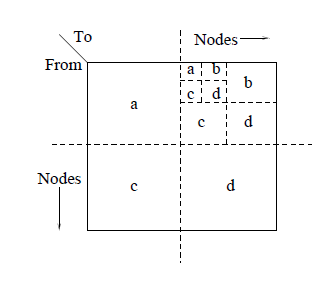
\includegraphics[scale=0.5]{/Rmat}
\caption{The R-mat model \cite{Rmat2004}}
\label{fig:Rmat}
\end{figure}

For this experiment, we set a global probability for activation at 5\% and an initial seed of 42 for the linear feedback shift register. We ran each information diffusion iteration 50 times and found the average coverage and time usage for each run; each run used a new initial seed, thus each run is different. 

Our implementation was a greedy solution, where the PS generated a new set of seeds. 

The processing system (PS) sends the matrix and frontier to the Processing logic (PL). The    

The implementation was done on a Zedboard \cite{ZedSpec}, with a ZYNQ7 Processing system. The adjacency matrix was stored in the 4GB SD card. The Zedboard was using a 15000000 JTAG Clock Frequency. 



\section{Results}
In Table \ref{ta:Vary buffer size}, we can see that by varying the buffer size, we get variable results. We can see that in C simulation, by using a larger buffer so that the IP core can take the entire row of the matrix, the result is somewhat better than the other. While for the RTL implementation, there does not seem to be the case. For the RTL simulation, by choosing buffer size equal to eight, get a better time. 

For table \ref{tab:Different K}, the first column shows the how many vertices were in the seed nodes, the second column displays the coverage. Unsurprisingly, the more seed nodes that were chosen, the larger was the coverage. For table \ref{tab:Different K}, the measurements are in microseconds.  The time usage(diffusion) column shows us how much time was spent on an average ICM iteration, while the last column shows how much time each seed selection took.

For Table \ref{tab:Software Different K}, it's the same experiments in software C simulation. The results are measured in seconds. 

\begin{table}[ht]
\centering
\caption{Results from Zedboard, different sized seed nodes.}
\label{tab:Different K}
\begin{tabular}{| >{\centering\arraybackslash}m{0.5in} |  >{\centering\arraybackslash}m{0.7in} |  >{\centering\arraybackslash}m{1.0in} |  >{\centering\arraybackslash}m{1.0in}|} 
\hline
 k     & coverage     &  Time usage(diffusion)in microseconds & Seed selection time usage in micro sec \\ \hline
 1  &         0.198750             &     32.74 us  & 0.45 us \\ \hline
 2  &         0.247500             &     936.88 us &    0.87 us \\ \hline
 3  &         0.306250            &     1237.62 us &   1.26 us     \\ \hline
 4  &         0.391250            &     1501.96 us &   1.63 us     \\ \hline
 5  &         0.460000            &     1936.74 us &    1.97 us \\ \hline
\end{tabular}
\end{table}



\begin{table}[ht]
\centering
\caption{Results from C simulation, different sized seed nodes.}
\label{tab:Software Different K}
\begin{tabular}{| >{\centering\arraybackslash}m{0.5in} |  >{\centering\arraybackslash}m{0.7in} |  >{\centering\arraybackslash}m{1.0in} |  >{\centering\arraybackslash}m{1.0in}|} 
\hline
 k     & coverage     &  Time usage(diffusion) & Time usage(seed) \\ \hline
 1  &         0.222500            &      0.000680 s     &  0.472000 s \\ \hline
 2  &         0.270000             &    0.000900 s &   1.209000 s \\ \hline
 3  &         0.307500            &     0.004400 s &  10.443000s     \\ \hline
 4  &         0.368750           &    0.005720 s & 13.901000 s     \\ \hline
 5  &         0.482500           &     0.004560 s &   16.497999 s \\ \hline
\end{tabular}
\end{table}


from these results, we can clearly see that the RTL simulation is faster then the C simulation.
\begin{table}[]
\centering
\caption{Results from simulation with vary buffer size}
\label{ta:Vary buffer size}
\begin{tabular}{| >{\centering\arraybackslash}m{0.7in} |  >{\centering\arraybackslash}m{1.2in} |  >{\centering\arraybackslash}m{1.2in} |} 
\hline
Buffersize & Time in milliseconds (with C simulation) & Time in milliseconds (with RTL simulation)\\ \hline
 4  &         7.200 ms            &     0.920 ms \\ \hline
 8  &         6.260 ms            &     0.680 ms     \\ \hline
 16    &          5.180 ms            &     0.760 ms     \\
\hline
\end{tabular}
\end{table}

\section{Performance}
As we can see, the hardware implementation is better than the C-simulated implementation, even at this low scale, we can see that the



We have here included a snapshot of our synthesis report. As we can see, we have a rather large usage of \textit{look-up table} (LUT) and \textit{flip-flop}(FF) for our design. This is the result of the PIPELINE and Loop unrolling. Our high-level implementation does contain several Loops and dependencies; this results in a significant amount of resource used. 


By using the random() function provided by Python, we placed '1' in its designated position. After the matrix was generated, we further applied a diagonal copying as shown in Figure:\ref{fig:flipDiagonal}. This is obligatory to create an undirected graph.



\section{Discussion}

\subsection{Results}
From our results its hard to say if HLS was an improvement or not. Since we worked on a network of such small scale, it is hard to say anything concrete regarding the effectiveness to HLS and our implementation. From the simulated data, we can see that C simulation is much slower than the hardware implementation. One reason that we got odd numbers might be that the testbench program that the C simulation used were slightly different than the FPGA.  

But the result from Table \ref{tab:Software Different K} is interesting. We can see that the seed selection algorithm was severely worse then the HLS implementation on FPGA. 

\subsection*{Analysis of the performance}
Our IP core was originally designed for networks with 1024 vertices, but after implementing with the optimization directives, the resource usage was massive. This resulted in a severe scale down for this project. The resulted network was reduced down to the size of 16 vertices. In network analysis, this is such a small scale that the results from this experiment would not be reliable. Since in such a small graph there might be multiple different factors can affect the results.  

The original idea with table \ref{ta:Vary buffer size} was to observe how the IP-core behaved when it would receive part of the matrix row. By finding an optimal buffer size that would satiate the bandwidth and still receive enough elements to compute. The result we got was not very representative. Since our implementation and the matrix we used was so small compared to other networks, we would not have been close to satiate the bandwidth.
 
In Figure 5.2, we can see that by synthesis an IP-core with several 1024 buffers, the resource estimate would be 222\% of the available LUT. This is due to our implementation have several large for and while loops. By including PIPELINE directive and UNROLL directive, results in significantly larger usage of resources then a core with a smaller buffer. 


\begin{figure}[!ht] \label{fig:synthesiseReport1024}
       \centerline{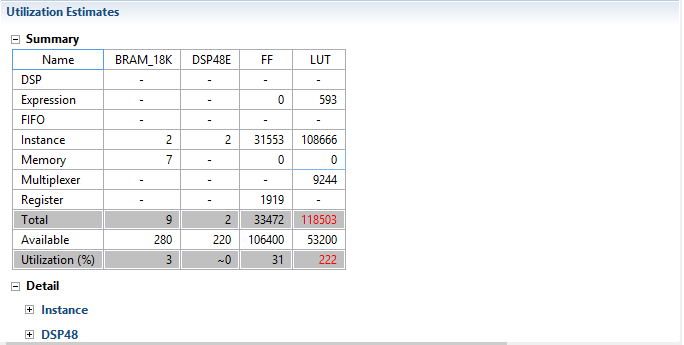
\includegraphics[scale=0.6]{Figures/SynthesisReport_1024}}
    \caption{Synthesis report for IP-core with buffersize 1024}
\end{figure}

Figure 5.3 is the synthesis report from our implementation with buffer size 16. The resource usage is much more realistic to what we can implement compared to Figure 5.2.

 \begin{figure}[!ht] \label{fig:synthesiseReport16}
      \centerline{ 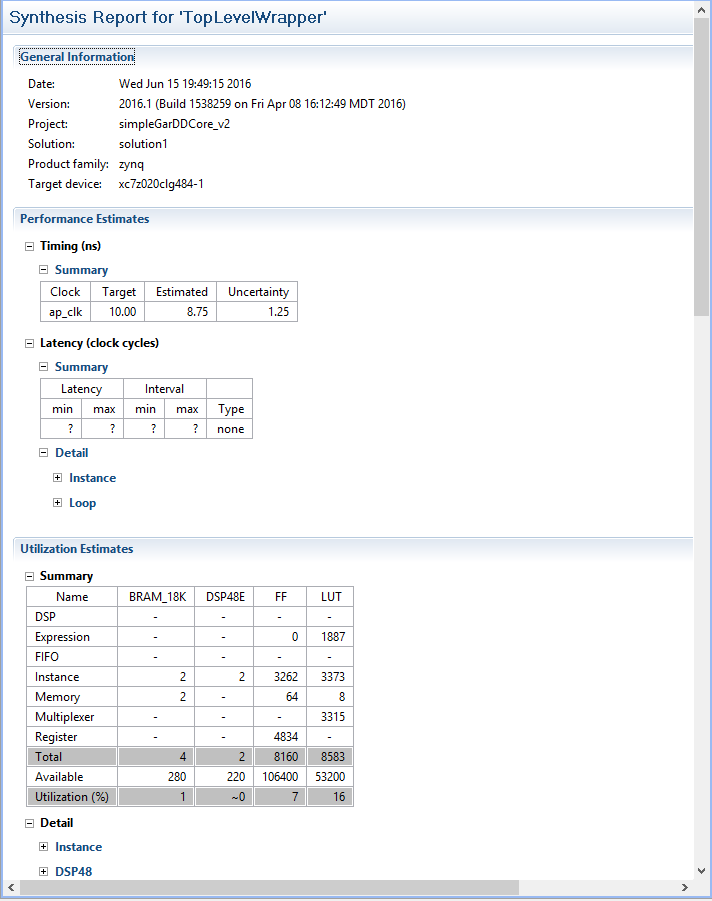
\includegraphics[scale=0.6]{Figures/SynthesisReport_16}}
    \caption{Synthesis report for IP-core with buffer size 16}
\end{figure}

 
\subsection*{problem that was encountered}
One problem that was encountered during this project was that the output signal from the synthesiser was not the correct direction. The output signal was often set as an input signal. The HLS would automatically set the values as output signal or input signal.The return value from a function would be set as an output signal, while the variable that the function takes would be set as the input signal. Another way to specify that something is the output signal would be to explicitly set them as pointer arguments. This will in set the signal to be the output signal.

Another problem that I often encountered was that the Vivado HLS often stop working. The problem was fixed by creating a new project and include the previous files.

Sometimes Vivado HLS was not able to Cosimulate the implementation the first time. I was not able to find a solution to this issue except resynthesis the project, which usually works.

There was an incidence where the implementation on the Zedboard did not behave as the implementation. This was solved by reprogramming the device and sometimes, restarting the Zedboard.
